\documentclass[11pt,letter]{article}
\usepackage[top=0.65in,bottom=0.9in,left=0.85in,right=0.85in]{geometry}

%\def\baselinestretch{1.25}
\def\baselinestretch{1.0}

\usepackage[greek, english]{babel}
\usepackage{multicol}

\usepackage{graphicx}
\usepackage[export]{adjustbox}


% The use of the times package forces the use of the type-1 times
% roman font, but the times roman font does not look nice.
% Besides the times roman font still does not print correctly on
% the dopy printer.
%\usepackage{times}


\usepackage{fancyhdr}
\usepackage{amsmath}
\usepackage{amssymb}
\usepackage{bm}
\usepackage{bbold}
\usepackage{parskip}
\usepackage{url}
\usepackage{xfrac}
\usepackage{isomath}

\newcommand{\bv}[1]{\ensuremath{\bm{#1}}}
\newcommand{\ts}[1]{\ensuremath{\tensorsym{#1}}}
\newcommand{\vo}{\ensuremath{V_{0}}}
\newcommand{\bvo}{\ensuremath{\bv{V}_{0}}}
\newcommand{\er}{\ensuremath{E_{R}}}

\newcommand{\efield}{\ensuremath{\bv{\mathcal{E}}}}
\newcommand{\efieldo}{\ensuremath{\mathcal{E}_{0}}}
\newcommand{\epspol}{\ensuremath{\hat{\bv{\varepsilon}}}}
\newcommand{\dpol}{\ensuremath{\bv{\mathrm{P}}}}

\newcommand{\Lc}{\ensuremath{L_{\mathrm{c}}}}
\newcommand{\dsig}[1]{\ensuremath{ \frac{ d\,\sigma_{#1} }{d\,\Omega} }}
\newcommand{\dbl}{\ensuremath{ \uparrow\! \downarrow \, }}
\newcommand{\spup}{\ensuremath{ \uparrow }}
\newcommand{\spdn}{\ensuremath{ \downarrow}}
%\newcommand{\hhh}{\ensuremath{\left( \sfrac{1}{2}\,\sfrac{1}{2}\,\sfrac{1}{2}\right)  }}
\newcommand{\hhh}{\ensuremath{\left( \frac{1}{2}\,\frac{1}{2}\,\frac{1}{2}\right)  }}

\begin{document}

{\Large \bf Polarization phase-contrast imaging}

In this document we will introduce the technique of polarization phase-contrast
imaging (PPCI), which is used at various stages of our experiment to measure
the in-situ column density of the dilute gas.   The general goal of atom
cloud imaging is to obtain a quantitative measure of the density distribution
of the sample by looking at the intensity, phase and polarization profiles of
light that has gone through it.    The widely used absorption imaging
technique looks at the intensity attenuation profile for a resonant, or nearly
resonant laser beam.   On the other hand, light with a larger detuning is used
for PPCI; rather than looking for attenuation of the intensity, the information
about the density of the gas can be extracted from the phase profile of the
transmitted beam.   The treatment is separated into four parts, first we
calculate how the light is affected by the polarized atomic cloud.  This is
done classicaly, using Maxwell's equations and assuming that we know the
polarization of the medium.  In the second part we calculate the general
polarization of the atomic cloud, which results from the perturbation on the
atoms by the oscillating electric field of the light. This culminates in the
determination of the electric susceptibility tensor.  In the third part we
evaluate the elements of the suceptibility tensor for the atomic structure that
is of interest in our application, namely a spin-mixture of $^{6}$Li atoms at
high magnetic field.  We then proceed to derive expressions that relate the
phase profile of the transmitted beam to the column density of the cloud.
In the fourth part we examine the experimental setup which allows one to
convert the phase profile into an intensity profile that can be recorded on a
CCD camera.  
 
\section{Transmission of light through a polarized gas} 

The electric field of the light that traverses the atomic cloud can be written
in general form (see Sec.~6.1 of~\cite{auzinsh2010optically}) as 
\begin{equation}
 \efield( \bv{r}, t ) = 
     \text{Re}\lbrace \efieldo e^{i(\bv{k}\cdot\bv{r} - \omega t + \varphi )} 
     [ \cos\alpha \bv{\hat{e}}_{1} 
   +   \sin\alpha e^{i\phi} \bv{\hat{e}}_{2} ] \rbrace 
  %\label{eq:efield-param}
\end{equation}

\begin{equation}
 \efield( \bv{r}, t ) = 
     \text{Re}\lbrace \efieldo e^{i(\bv{k}\cdot\bv{r} - \omega t + \varphi )} 
     [ ( \cos\alpha \cos \epsilon - i \sin\alpha\sin\epsilon) \bv{\hat{e}}_{1} 
   + (\sin\alpha \cos\epsilon + i \cos\alpha\sin\epsilon) \bv{\hat{e}}_{2} ] \rbrace 
  \label{eq:efield-param}
\end{equation}
where $\bv{\hat{e}}_{1,2}$ are two orthogonal unit vectors perpendicular to the
wave vector $\bv{k}$ and perpendicular to each other,  $\efieldo$ is the
electric field amplitude, $\varphi$ is an overall phase,  $\alpha$ is the angle
between the major axis of the polarization ellipse and the $\bv{\hat{e}}_{1}$
axis, and $\epsilon$ is the arctangent of the ratio of the minor to the major
axis of the polarization ellipse. 

The wave equation in a dielectric medium can be obtained from Maxwell's
equations (see Sec.~10.1 of~\cite{auzinsh2010optically}), and is given by
\begin{equation}
 \nabla^{2} \efield 
 -\frac{1}{c^{2}} \frac{\partial^{2} \efield } {\partial t^{2}} 
  = \frac{4\pi}{c^{2}} \frac{\partial^{2} \dpol }{\partial t^{2} } 
\end{equation} 
here the medium polarization $\dpol$ (which is induced by the light)
corresponds to the dipole moment per unit volume.   If we know the dipole
moment of a single atom $\langle d \rangle$ then \begin{equation}
 \dpol = n \langle d \rangle 
\end{equation}
where $n$ is the density of the gas.

Just as the electric field was parameterized in Eq.~\ref{eq:efield-param}, the
same can be done with the polarization in terms of the four real parameters
$P_{i}$ as 
\begin{equation}
 \dpol = \text{Re} \lbrace e^{i(\bv{k}\cdot\bv{r} - \omega t + \varphi) }
   [(P_{1} - i P_{2}) \bv{\hat{e}}_{1} + ( P_{3} - i P_{4}) \bv{\hat{e}}_{2} ] \rbrace
  \label{eq:pol-param}
\end{equation}

Using the oscillatory time dependence of \efield\ and \dpol\ the wave equation
is reduced to 
\begin{equation}
   \frac{ \partial^{2} \efield}{\partial \ell^{2} }  + k^{2} \efield = - 4 \pi k^{2} \dpol
\end{equation}
where $\ell$ is the distance along the light propagation direction. 

The parameterized electric field and polarization are plugged into the wave
equation,  and one proceeds to neglect terms that are of second order in the
derivatives of the electric field parameters.  This justifiable as long as the
fractional change of the parameters is small over one wavelength of the light,
which is certainly the case for our dilute atom cloud.  The resulting
expressions for the change of the field parameters per unit distance are:
\begin{align}
 \frac{1}{\efieldo} \frac{d \efieldo }{ d \ell} =  
     \frac{2\pi \omega}{\efieldo c} ( P_{2} \cos\alpha + P_{4} \sin\alpha ) \\ 
 \frac{ d \varphi }{d \ell} = 
     \frac{2\pi\omega}{\efieldo c} \left( \frac{ P_{1} }{\cos\alpha} \right) \\
 \frac{ d \alpha}{ d \ell} = 
     \frac{2\pi\omega}{\efieldo c} ( -P_{2} \sin\alpha + P_{4} \cos\alpha ) \\
 \frac{ d \phi}{ d \ell} = 
     - \frac{2\pi\omega}{\efieldo c }
     \left(  \frac{ -P_{1}\sin\alpha + P_{3}\cos\alpha }{ \sin\alpha\cos\alpha } \right)
\end{align}
%\begin{align} 
% \frac{1}{\efieldo} \frac{d \efieldo }{ d \ell} =  
%     \frac{2\pi \omega}{\efieldo c} [ \sin\alpha( -P_{1} \sin\epsilon 
%          + P_{4} \cos\epsilon) + \cos\alpha( P_{2} \cos\epsilon + P_{3} \sin\epsilon) ] \\
% \frac{ d \varphi }{d \ell} = 
%     \frac{2\pi\omega}{\efieldo c} \sec 2 \epsilon[ 
%         \cos\alpha( P_{1} \cos\epsilon + P_{4}\sin\epsilon) + 
%         \sin\alpha( -P_{2}\sin\epsilon + P_{3}\cos\epsilon) ] \\
% \frac{ d \alpha}{ d \ell} = 
%     \frac{2\pi\omega}{\efieldo c} \sec 2 \epsilon[
%         \cos\alpha( P_{1} \sin\epsilon + P_{4}\cos\epsilon) -
%         \sin\alpha( P_{2}\cos\epsilon - P_{3}\sin\epsilon) ] \\
% \frac{ d \epsilon}{ d \ell} = 
%     - \frac{2\pi\omega}{\efieldo c }[ \sin\alpha
%         (P_{1} \cos\epsilon + P_{4} \sin\epsilon) 
%       + \cos\alpha ( P_{2} \sin\epsilon - P_{3} \cos\epsilon ) ]
%\end{align}
\begin{align} 
 \frac{1}{\efieldo} \frac{d \efieldo }{ d \ell} =  
     \frac{2\pi \omega}{\efieldo c} [  
          - P_{1} \sin\alpha\sin\epsilon 
          + P_{4} \sin\alpha\cos\epsilon
          + P_{2} \cos\alpha\cos\epsilon 
          + P_{3} \cos\alpha\sin\epsilon ] \\
 \frac{ d \varphi }{d \ell} = 
     \frac{2\pi\omega}{\efieldo c} \sec 2 \epsilon[ 
            P_{1} \cos\alpha\cos\epsilon 
          + P_{4} \cos\alpha\sin\epsilon
          - P_{2}\sin\alpha\sin\epsilon 
          + P_{3}\sin\alpha\cos\epsilon ] \\
 \frac{ d \alpha}{ d \ell} = 
     \frac{2\pi\omega}{\efieldo c} \sec 2 \epsilon[
            P_{1} \cos\alpha\sin\epsilon 
          + P_{4} \cos\alpha\cos\epsilon
          - P_{2} \sin\alpha\cos\epsilon 
          + P_{3} \sin\alpha\sin\epsilon ] \\
 \frac{ d \epsilon}{ d \ell} = 
     - \frac{2\pi\omega}{\efieldo c }[ 
            P_{1} \sin\alpha\cos\epsilon 
          + P_{4} \sin\alpha\sin\epsilon
          + P_{2} \cos\alpha\sin\epsilon 
          - P_{3} \cos\alpha\cos\epsilon  ] 
 \label{eq:diff-param} 
\end{align}
 
     
    
\section{Polarization of the cloud}  


If we can calculate the electric
dipole moment induced on one atom, $\langle \bv{d}\, \rangle$, and if we know
the density of the cloud, $n(\vec{r})$, then we can simply write the induced
polarization as 
\begin{equation}
 \dpol(\bv{r}) = \langle \bv{d}\, \rangle n(\bv{r}) 
\end{equation}

An ensemble of atoms (in which each atom may be in a different quantum state) is
best described using the density matrix, which is defined as \begin{equation}
  \rho = \frac{1}{N} \sum_{i=1}^{N} | \psi_{i} \rangle \langle \psi_{i} | 
\end{equation}
where the $i^{\text{th}}$ atom in the ensemble is in state $|\psi_{i}\rangle$.
The expectation value of the electric dipole moment is then given by 
\begin{equation}
\begin{split}
   \langle \bv{d}\, \rangle  & = \text{Tr} ( \rho \bv{d} )  \\
   & = \sum_{mn} \rho_{mn} \langle n | \bv{d} | m \rangle
\end{split} 
\end{equation} 
Since the dipole operator only couples states of different parity, the terms
that contribute to this sum correspond to $m,n$ being a ground and excited
state pair.   

The equation of motion for the density matrix follows from the Schrodinger
equation for the $|\psi_{i}\rangle$,  it is known as the Liouville equation,
which, including the spontaneous decay of the excited state, 
is~\cite{auzinsh2010optically} 
\begin{equation}
  i \hbar \dot{\rho} = 
  [H, \rho] - \frac{i\hbar}{2}\lbrace \hat{\Gamma}, \rho \rbrace + i\hbar\text{Tr}( F \rho ) 
\end{equation}
where $\hat{\Gamma}$ is the relaxation matrix, a diagonal matrix with the decay
rate of each state on the diagonal (see Sec.~5.5
in~\cite{auzinsh2010optically}), and $F$ is the spontaneous emission operator
(see Sec.~12.1 in~\cite{auzinsh2010optically}).  The hamiltonian
$H$ can be split into a diagonal part, $H_{0}$, which includes the
level structure of the atom in the presence of a magnetic field, and the time
dependent perturbation from the electric field $\hbar V$:
\begin{equation}
  H = H_{0} + \hbar V
\end{equation}

The matrix element $\rho_{ge}$, where $g$, $e$ represent a ground and an
excited state respectively, satisfies
\begin{equation}
\begin{split}
  \dot{\rho}_{ge}  & =  
   \frac{1}{i\hbar} \langle g | [ H_{0}, \rho ] | e \rangle  
 - i \langle g | [ \hbar V, \rho ] | e \rangle 
 - \frac{1}{2}\langle g | \lbrace \hat{\Gamma}, \rho \rbrace | e \rangle 
 + \langle g | \text{Tr}( F \rho ) | e \rangle  \\
 & = -i \tilde{\omega}_{ge}  \rho_{ge}  
     -i \sum_{p}\left( V_{gp} \rho_{pe} - \rho_{gp}V_{pe} \right) 
     +  \sum_{rs} F_{ge}^{sr} \rho_{rs}
\end{split} 
\end{equation}
where 
\begin{equation}
  \tilde{\omega}_{ge} = (E_{g} - E_{e})/\hbar - i \Gamma_{e} /2 
\end{equation}
We notice that $F_{ge}^{sr} = 0$, since $F$ is only nonzero if the lower
indices are both ground states and the upper indices are both excited states.
So we are left with 
\begin{equation}
  \dot{\rho}_{ge}  =  
     -i \tilde{\omega}_{ge}  \rho_{ge}  
     -i \sum_{p}\left( V_{gp} \rho_{pe} - \rho_{gp}V_{pe} \right) 
\end{equation}

At this point we switch to the rotating frame (see Sec.~10.2.2
in~\cite{auzinsh2010optically}), in which the density matrix $\tilde{\rho}$ can
be obtained from
\begin{equation}
 \tilde{\rho} = U^{\dagger} \rho U
\end{equation} 
where $U$ is a unitary diagonal matrix given by 
\begin{equation} 
  U_{mm} = \begin{cases} 
   1 & \text{if  $m$ is a ground state} \\
   e^{i(\bv{k}\cdot\bv{r}-\omega t)} & \text{if $m$ is an excited state} 
  \end{cases}
\end{equation}
We thus have $\tilde{\rho}_{ge} = \rho_{ge} e^{i(\bv{k}\cdot\bv{r}-\omega t)}$, and the equation
of motion for the matrix element in the rotating frame is
\begin{equation}
\begin{split}
  \dot{\tilde{\rho}}_{ge} & = 
     -i\omega \tilde{\rho}_{ge} + \dot{\rho}_{ge} e^{i(\bv{k}\cdot\bv{r}-\omega t)} \\
     &  =  
     -i\omega \tilde{\rho}_{ge} + 
      \left[ 
     -i \tilde{\omega}_{ge}  \rho_{ge}  
     -i \sum_{p}\left( V_{gp} \rho_{pe} - \rho_{gp}V_{pe} \right) 
      \right] e^{i(\bv{k}\cdot\bv{r}-\omega t)}  \\ 
     &  =  
     -i \tilde{\rho}_{ge}\tilde{\omega}'_{ge}   
     -i \sum_{p}\left( V_{gp} \rho_{pe} - \rho_{gp}V_{pe}\right)  e^{i(\bv{k}\cdot\bv{r}-\omega t)}   
\end{split} 
\end{equation}
where 
\begin{equation}
  \tilde{\omega}'_{ge} = \omega + (E_{g} - E_{e})/\hbar - i \Gamma_{e}/2 
   \equiv  \Delta_{ge} - i \Gamma_{e}/2 
\end{equation}
We recall that the interaction term is given by 
\begin{equation} 
  \hbar V = -\bv{d} \cdot \efield 
    =  -\bv{d} \cdot \efieldo \text{Re}[ \epspol e^{i(\bv{k}\cdot\bv{r} - \omega t )} ]
    =  -\bv{d} \cdot \frac{  \efieldo ( \epspol e^{i(\bv{k}\cdot\bv{r} - \omega t)} 
                             + \epspol^{*} e^{-i(\bv{k}\cdot\bv{r}-i\omega t)} )}{2}  \end{equation}
Introducing this in the equation of motion for $\tilde{\rho}_{ge}$, 
neglecting the rapidly oscillating terms, and making use of the fact that the
wavelength of the light is much larger than the extent of the atom (so that the
spatially dependent exponential can be taken outside of matrix elements) one
gets to 
\begin{equation} 
\begin{split}
  \dot{\tilde{\rho}}_{ge} & =  
     -i \tilde{\rho}_{ge}\tilde{\omega}'_{ge}   
     + \frac{i}{2\hbar} \sum_{p}\left[ \bv{d}_{gp} \rho_{pe} 
     - \rho_{gp}\bv{d}_{pe}\right] \cdot \efieldo \epspol^{*}
\end{split} 
\end{equation}
which has a steady-state solution given by 
\begin{equation} 
  \tilde{\rho}_{ge}  = \frac{1}{2 \hbar\tilde{\omega}'_{ge} }  
       \sum_{p}\left[ \bv{d}_{gp} \rho_{pe} 
     - \rho_{gp}\bv{d}_{pe}\right] \cdot \efieldo \epspol^{*}
\end{equation}
Finally, we neglect coherences and populations in the excited states
($\rho_{ee'}=0$) and coherences in the ground states ($\rho_{gg'}=0$ if $g\neq
g'$).   This can be justified since the perturbation is week and is not
expected to modify the initial excited state populations (which are zero).
Furthermore, coherences between ground states $g\neq g'$ can only be expected
if there is  population in the excited state.  These coherences
can only develop is there is excitation from one ground state and then
spontaneous or stimulated emission to a different ground state, so they
can be neglected in the weak perturbation treatment.  The final result is 
\begin{equation} 
  \tilde{\rho}_{ge} 
  =  -\frac{\bv{d}_{ge} \cdot \efieldo \epspol^{*}  }
       {\hbar (2 \Delta_{ge} - i \Gamma )} \rho_{gg} 
\end{equation}
%\begin{equation} 
%  \Rightarrow  \ \ \ 
%  \rho_{ge}  = -\frac{1}{2 \tilde{\omega}'_{ge} }  
%       (\bv{d}_{ge} \cdot \efield) e^{i\omega t}
%\end{equation}
which after plugging back into the equation for the expectation value of the dipole
moment gives 
\begin{equation}
\begin{split}
   \langle \bv{d}\, \rangle 
   & = \sum_{ge} 2 \text{Re}[ \rho_{ge} \bv{d}_{eg} ] \\
   & = \sum_{ge} 2 \text{Re}[ \tilde{\rho}_{ge}e^{-i(\bv{k}\cdot\bv{r}-\omega t)}\bv{d}_{eg} ]   \\
   & = \sum_{ge} \rho_{gg}\text{Re}[ 
 -\frac{\bv{d}_{ge} \cdot \efieldo \epspol^{*} }{ \hbar( \Delta_{ge} + i \Gamma/2 )} 
   e^{-i(\bv{k}\cdot\bv{r} - \omega t) } 
 \bv{d}_{eg} ]   \\
   & \equiv \sum_{ge}  \rho_{gg} \text{Re}[ 
 -\frac{\bv{d}_{eg} \cdot \efieldo \epspol }{ \hbar( \Delta_{ge} -i \Gamma/2 ) } 
   e^{i(\bv{k}\cdot\bv{r} - \omega t) } 
 \bv{d}_{ge} ]   \\
   & = \sum_{ge}  \rho_{gg}  \text{Re}[ 
 -\frac{\bv{d}_{eg} \cdot \tilde{\efield} }{ \hbar(  \Delta_{ge} -i \Gamma/2 ) } 
 \bv{d}_{ge} ]   \\
\end{split} 
\end{equation}
where in the last line $\tilde{\efield}= \efieldo \hat{\bv{\varepsilon}}
e^{i(\bv{k}\cdot\bv{r} - \omega t)}$ is the complex electric field vector (not
to be confused with the actual electric field vector, which is the real part of
it).

Labeling the cartesian components of $\bv{d}$ with greek upper
indices and implying sums over repeated greek indices, we have  
\begin{equation}
\begin{split}
   \langle d^{\mu} \rangle
   & = \sum_{ge}   \rho_{gg}  \text{Re}[ -\frac{d_{eg}^{\nu} \tilde{\mathcal{E}}^{\nu}  d_{ge}^{\mu} }
      { \hbar(\Delta_{ge} - i\Gamma/2) }    ] \\
   & = \text{Re}\left[ \left( \sum_{ge}- \rho_{gg} \frac{d_{eg}^{\nu}   d_{ge}^{\mu}  }
       { \hbar(\Delta_{ge} - i\Gamma/2) }   
       \right)  \tilde{\mathcal{E}}^{\nu} \right] 
\end{split}
\end{equation}
and from here we can write 
\begin{equation}
   \dpol = \text{Re}\left[ \epsilon_{0} \ts{\chi} \tilde{ \efield }  \right] \\
\end{equation}
where we have defined the electric susceptibility tensor as
\begin{equation}
\begin{split}
   \chi_{\mu\nu}
   & = - \frac{n}{\hbar\epsilon_{0}} \sum_{ge}\rho_{gg} \frac{d_{eg}^{\nu}   d_{ge}^{\mu}  }
       { \Delta_{ge} - i\Gamma/2 } \\ 
   & = - \frac{n}{\hbar\epsilon_{0}} \sum_{ge}\rho_{gg} 
   \frac{\langle e | d^{\nu} | g \rangle \langle g | d^{\mu} | e \rangle } 
       { \Delta_{ge} - i\Gamma/2 } 
\end{split} 
\end{equation}


\section{Susceptibility for $^{6}$Li atoms at high magnetic field}

Going back to the parameterization scheme introduced in
Eqs.~\ref{eq:efield-param},\ref{eq:pol-param} we can identify\footnote{
The reader is reminded that $\ts{\chi}$ is a tensor and, for instance, the
prodcuct $\ts{\chi} \bv{\hat{e}}_{1}$ may have components along both
$\bv{\hat{e}}_{1}$ and $\bv{\hat{e}}_{2}$.}
\begin{equation}
   (P_{1} - i P_{2}) \bv{\hat{e}}_{1} + ( P_{3} - i P_{4}) \bv{\hat{e}}_{2} 
 =  \epsilon_{0} \efieldo \ts{\chi} 
     [  \cos\alpha  \bv{\hat{e}}_{1} 
   + \sin\alpha e^{i\phi}  \bv{\hat{e}}_{2} ] 
\end{equation}
\begin{equation}
   (P_{1} - i P_{2}) \bv{\hat{e}}_{1} + ( P_{3} - i P_{4}) \bv{\hat{e}}_{2} 
 =  \epsilon_{0} \efieldo \ts{\chi} 
     [ ( \cos\alpha \cos \epsilon - i \sin\alpha\sin\epsilon) \bv{\hat{e}}_{1} 
   + (\sin\alpha \cos\epsilon + i \cos\alpha\sin\epsilon) \bv{\hat{e}}_{2} ] 
\end{equation}

Using  
$\bv{\hat{e}}_{1} = \left[ \begin{smallmatrix}  1 \\ 0 \end{smallmatrix} \right]$
and 
$\bv{\hat{e}}_{2} = \left[ \begin{smallmatrix}  0 \\ 1 \end{smallmatrix} \right]$
this can be written in matrix form as 
\begin{equation}
 \left[ \begin{matrix}  P_{1}-iP_{2} \\ P_{3}-iP_{4} \end{matrix} \right]
  =  \epsilon_{0}\efieldo 
 \left[ \begin{matrix}
     \chi_{11} & \chi_{12} \\ \chi_{21} & \chi_{22} 
 \end{matrix} \right]
 \left[ \begin{matrix}
      \cos\alpha \\
      \sin\alpha e^{i\phi}
 \end{matrix} \right]
\end{equation}
\begin{equation}
 \left[ \begin{matrix}  P_{1}-iP_{2} \\ P_{3}-iP_{4} \end{matrix} \right]
  =  \epsilon_{0}\efieldo 
 \left[ \begin{matrix}
     \chi_{11} & \chi_{12} \\ \chi_{21} & \chi_{22} 
 \end{matrix} \right]
 \left[ \begin{matrix}
      \cos\alpha \cos \epsilon - i \sin\alpha\sin\epsilon \\
      \sin\alpha \cos\epsilon + i \cos\alpha\sin\epsilon
 \end{matrix} \right]
\end{equation}

At this point we have to make a choice for the vectors $\bv{\hat{e}}_{1,2}$.
In our imaging setup the magnetic field is oriented along the $z$ axis, and the
probe beam propagate along $y$, perpendicular to the magnetic field.   The
polarization of the light lies on the xz plane, so we will asign
$\bv{\hat{e}}_{1} = \bv{\hat{x}}$ and $\bv{\hat{e}}_{2} = \bv{\hat{z}}$, and we
will evaluate the corresponding components of the electric susceptibility
tensor: $\chi_{xx}$, $\chi_{xz}$, $\chi_{zx}$, and $\chi_{zz}$.

The first thing to notice is that the off diagonal components of the
susceptibility vanish.  This is because the $x$ and $z$ components of the
dipole cannot couple to thesame excited state.   For the diagonal components we
will need to evaluate the matrix elements $ | \langle e | d_{x,z} | g \rangle
|^{2} $,  which can be expressed in terms of the spherical basis components of
the dipole moment, $d_{q}$, as 
\begin{align}
|\langle e | d_{i} | g \rangle|^{2} & =  \sum_{q} |\bv{\hat{e}}_{i}\cdot \bv{\hat{e}}_{q}|^{2} 
 | \langle e | d_{q} | g \rangle | ^{2} 
\end{align}

We recall that the relevant quantum numbers for the ground and excited states are
\begin{align}
|g\rangle & = | R_{g}\, L\,S\,J\,m_{J} \rangle \\
|e\rangle & = | R_{e}\, L\,S\,J\,m_{J} \rangle \\
\end{align}
At the field of interest, the nuclear spin and its projection are decoupled
from the angular momentum of the electron,  so they do not play any role in the
atomic transition.
\begin{figure}[h]
\centering 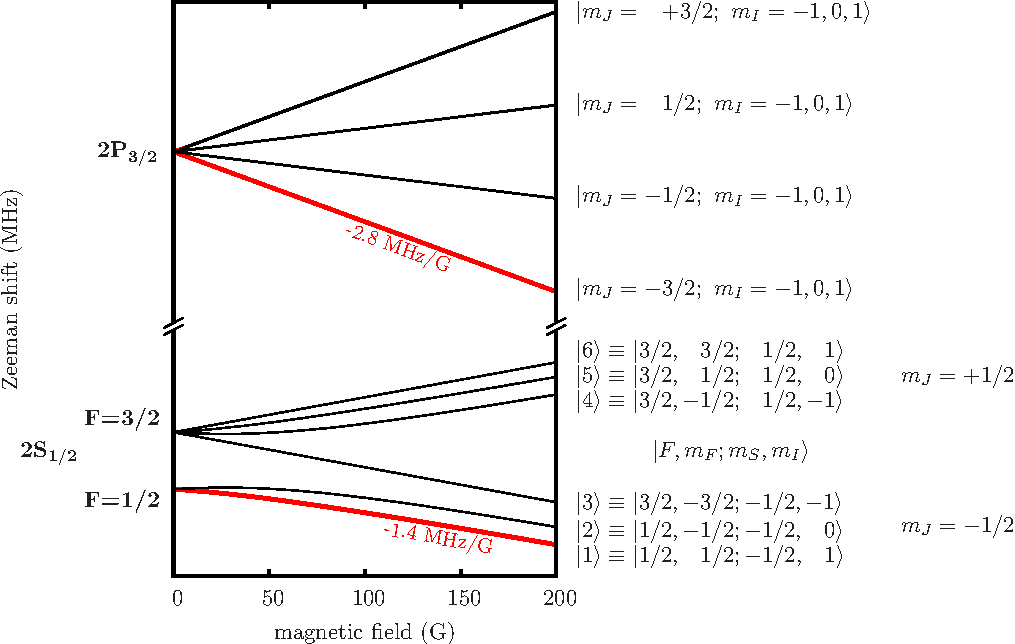
\includegraphics[width=0.85\textwidth]{01eps.pdf}
\caption[Levels relevant for imaging.]{Level diagram relevant for imaging transitions}  \label{fig:levels}
\end{figure}
Figure~\ref{fig:levels} shows the energy levels of the $2S_{1/2}$ and
$2P_{3/2}$ states of a $^{6}$Li atom in the presence of a magnetic field. In
our experiment we tipically have atoms in an incoherent spin mixure of states
$|1\rangle$ and $|2\rangle$.  Both of those state have $m_{J}=-1/2$ so from
either of them one can drive transitions to excited states with $m_{J}=-3/2,
-1/2, +1/2$.  In what follows we refer to those excited states $|e\rangle$ as
$|-\rangle$, $|\pi\rangle$, and $|+\rangle$ respectively. 

 
To evaluate $ | \langle e | d_{q} | g \rangle | ^{2} $, we use the
Wigner-Eckart theorem(see Sec.~5.4.1 of ~\cite{edmonds1996angular}) to make the
total angularm momentum selection rules explicit in a 3$j$-symbol.   This
defiens the reduced matrix element $|\langle R_{e}\, L\,S\,J || d || R_{g}\, L\,S\,J \rangle|^{2}$, 
\begin{align}
|\langle e | d_{q} | g \rangle|^{2} & = \begin{pmatrix} J_{e} & 1 & J_{g} \\ -m_{Je} & q & m_{Jg} \end{pmatrix}^{2}
|\langle R_{e}\, L\,S\,J || d || R_{g}\, L\,S\,J \rangle|^{2}
\end{align}
The dipole moment operator only acts on the electronic angular momentum, $L$,
and our quantum state is expressed in the $LS$ coupled scheme, where $L$ and
$S$ are coupled to form $J=L+S$.  One can use the formula for the expectation
of a single part operator on a coupled scheme (see Sec.~7.1.7 on
\cite{edmonds1996angular}), in this case the dipole moment operating on the
$LS$ coupled state. One obtains 
\begin{align}
|\langle e | d_{q} | g \rangle|^{2} & = \begin{pmatrix} J_{e} & 1 & J_{g} \\ -m_{Je} & q & m_{Jg} \end{pmatrix}^{2}
(2J_{e}+1)(2J_{g}+1)  \begin{Bmatrix}L_{g} & J_{g} & S \\ J_{e} & L_{e} & 1 \end{Bmatrix}^{2}|\langle R_{e}\, L || d || R_{g}\, L \rangle|^{2}
\end{align}
The fully reduced matrix element can be related to the lifetime, $\tau$, or the
natural linewidth, $\Gamma$, of the excited state~\cite{Olivares:98}, 
\[
|\langle R_{e}\, L || d || R_{g}\, L \rangle|^{2} = \frac{1}{\tau} \frac{ 9\epsilon_{0} \hbar \lambda^{3}}{8 \pi^{2}} = \Gamma\frac{ 9\epsilon_{0} \hbar \lambda^{3}}{8 \pi^{2}} \]
resulting finally in 
\begin{align}
|\langle e | d_{q} | g \rangle|^{2} & = \begin{pmatrix} J_{e} & 1 & J_{g} \\ -m_{Je} & q & m_{Jg} \end{pmatrix}^{2}
(2J_{e}+1)(2J_{g}+1)  \begin{Bmatrix}L_{g} & J_{g} & S \\ J_{e} & L_{e} & 1 \end{Bmatrix}^{2}\Gamma\frac{ 9\epsilon_{0} \hbar \lambda^{3}}{8 \pi^{2}}
\end{align}
At this point we plug in some of the values for our case, $L_{g}=0$, $J_{g} =
1/2$, $m_{Jg}=-1/2$, $L_{e}=1$, and $J_{e}=3/2$.  The $6j$ symbol can be
evaluated in Mathematica.  This results in, 
\begin{align}
|\langle e | d_{q} | g \rangle|^{2} & = \begin{pmatrix} J_{e} & 1 & J_{g} \\ -m_{Je} & q & m_{Jg} \end{pmatrix}^{2}
\Gamma\frac{ 3\epsilon_{0} \hbar \lambda^{3}}{2 \pi^{2}}
\end{align}
\begin{align}
|\langle e | d_{i} | g \rangle|^{2} & =  \sum_{q} |\bv{\hat{e}}_{i}\cdot \bv{\hat{e}}_{q}|^{2} \begin{pmatrix} J_{e} & 1 & J_{g} \\ -m_{Je} & q & m_{Jg} \end{pmatrix}^{2}
\Gamma\frac{ 3\epsilon_{0} \hbar \lambda^{3}}{2 \pi^{2}}
\end{align}

Going back to the $x$ and $z$ components of the dipole moment we have 
\begin{equation}
\begin{split}
   \chi_{xx}
   & = - \frac{n}{\hbar\epsilon_{0}} \sum_{ge}\rho_{gg} 
   \frac{ |\langle g | d_{x} | e \rangle|^{2} } 
       { \Delta_{ge} - i\Gamma/2 } \\
   & = - \frac{n}{\hbar\epsilon_{0}} \sum_{g} \rho_{gg} 
       \Gamma\frac{ 3\epsilon_{0} \hbar \lambda^{3}}{2 \pi^{2}} 
       \left( \frac{1}{\Delta_{-} - i \Gamma/2 } 
              |\bv{\hat{e}}_{x}\cdot \bv{\hat{e}}_{-}|^{2} 
              \begin{pmatrix} 3/2 & 1 & 1/2 \\ 3/2 & -1 & -1/2 \end{pmatrix}^{2} \right.  \\
   & \ \ \ \ \ \ \hspace{1.3in}\   +  
       \left. \frac{1}{\Delta_{+} - i \Gamma/2 } 
              |\bv{\hat{e}}_{x}\cdot \bv{\hat{e}}_{+}|^{2} 
              \begin{pmatrix} 3/2 & 1 & 1/2 \\ -1/2 & +1 & -1/2 \end{pmatrix}^{2} 
       \right) \\ 
   & = - \frac{n}{\hbar\epsilon_{0}} \sum_{g} \rho_{gg} 
       \Gamma\frac{ 3\epsilon_{0} \hbar \lambda^{3}}{2 \pi^{2}} 
       \left( \frac{1/8}{\Delta_{-} - i \Gamma/2 } 
       +  
              \frac{1/24}{\Delta_{+} - i \Gamma/2 }  
       \right)  
\end{split} 
\end{equation}
\begin{equation}
\begin{split}
   \chi_{zz}
   & = - \frac{n}{\hbar\epsilon_{0}} \sum_{ge}\rho_{gg} 
   \frac{ |\langle g | d_{z} | e \rangle|^{2} } 
       { \Delta_{ge} - i\Gamma/2 } \\
   & = - \frac{n}{\hbar\epsilon_{0}} \sum_{g} \rho_{gg} 
       \Gamma\frac{ 3\epsilon_{0} \hbar \lambda^{3}}{2 \pi^{2}} 
              \frac{1}{\Delta_{\pi} - i \Gamma/2 } 
              |\bv{\hat{e}}_{z}\cdot \bv{\hat{e}}_{0}|^{2} 
              \begin{pmatrix} 3/2 & 1 & 1/2 \\ 1/2 & 0 & -1/2 \end{pmatrix}^{2} \\
   & = - \frac{n}{\hbar\epsilon_{0}} \sum_{g} \rho_{gg} 
       \Gamma\frac{ 3\epsilon_{0} \hbar \lambda^{3}}{2 \pi^{2}} 
              \frac{1/6}{\Delta_{\pi} - i \Gamma/2 } 
\end{split} 
\end{equation}

In our experiment we have a 50/50 spin mixture of atoms in the ground states
$|1\rangle$ and $|2\rangle$,  so the sum over $\rho_{gg}$ can be carried out to
give 
\begin{equation}
\begin{split}
   \chi_{xx} & = - n  
       \Gamma\frac{ 3  \lambda^{3}}{2 \pi^{2}} 
       \left( \frac{1/8}{\Delta_{-} - i \Gamma/2 } 
       +  
              \frac{1/24}{\Delta_{+} - i \Gamma/2 }  
       \right)  \\
   \chi_{zz} & = - n
       \Gamma\frac{ 3 \lambda^{3}}{2 \pi^{2}} 
              \frac{1/6}{\Delta_{\pi} - i \Gamma/2 } 
\end{split}
\end{equation}

Returning to the polarization parameters we have 
\begin{equation}
\begin{split}
  P_{1} - i P_{2} & = \epsilon_{0} \efieldo \chi_{xx} \cos\alpha \\
  P_{3} - i P_{4} & = \epsilon_{0} \efieldo \chi_{zz} \sin\alpha e^{i\phi} \\
      & =   \epsilon_{0}\efieldo \sin\alpha \left[
            (\text{Re}\chi_{zz} \cos\phi - \text{Im}\chi_{zz}\sin\phi ) 
          +i(\text{Re}\chi_{zz} \sin\phi + \text{Im}\chi_{zz}\cos\phi ) \right]
\end{split}
\end{equation}
\begin{equation}
\begin{split}
  P_{1} - i P_{2} & = \epsilon_{0} \efieldo \chi_{xx}
      [\cos\alpha \cos \epsilon - i \sin\alpha\sin\epsilon] \\
  P_{3} - i P_{4} & = \epsilon_{0} \efieldo \chi_{zz} 
      [\sin\alpha \cos\epsilon + i \cos\alpha\sin\epsilon]
\end{split}
\end{equation}
which becomes
\begin{equation}
\begin{split}
  P_{1} &= \epsilon_{0} \efieldo \text{Re}\chi_{xx} \cos\alpha \\
  P_{2} &= -\epsilon_{0} \efieldo \text{Im}\chi_{xx} \cos\alpha \\ 
  P_{3} &= \epsilon_{0} \efieldo \sin\alpha 
            (\text{Re}\chi_{zz} \cos\phi - \text{Im}\chi_{zz}\sin\phi ) \\ 
  P_{4} &= -\epsilon_{0} \efieldo \sin\alpha
          (\text{Re}\chi_{zz} \sin\phi + \text{Im}\chi_{zz}\cos\phi ) \\ 
\end{split}
\end{equation}
\begin{equation}
\begin{split}
  P_{1} &= \epsilon_{0} \efieldo[
            ( \cos\alpha\cos\epsilon ) \text{Re}\chi_{xx}
          + ( \sin\alpha\sin\epsilon ) \text{Im}\chi_{xx} ]\\ 
  P_{2} &= \epsilon_{0} \efieldo[
            ( \cos\alpha\cos\epsilon ) \text{Im}\chi_{xx} 
          + ( \sin\alpha\sin\epsilon ) \text{Re}\chi_{xx} ]\\ 
  P_{3} &= \epsilon_{0} \efieldo[
            ( \sin\alpha\cos\epsilon ) \text{Re}\chi_{zz}
          - ( \cos\alpha\sin\epsilon ) \text{Im}\chi_{zz} ]\\
  P_{4} &= -\epsilon_{0} \efieldo[
            ( \sin\alpha\cos\epsilon ) \text{Im}\chi_{zz} 
          + ( \cos\alpha\sin\epsilon ) \text{Re}\chi_{zz} ]\\ 
\end{split}
\end{equation}
The ratio of the imaginary to the real part of the susceptibility components
goes as $\chi_{ii} \sim \Gamma / \Delta$.  In phase-contrast imaging the
detuning is chosen so that the imaginary part  can be neglected, which results
in
\begin{equation}
\begin{split}
  P_{1} &= \epsilon_{0} \efieldo \text{Re}\chi_{xx} \cos\alpha \\
  P_{2} &= 0\\ 
  P_{3} &= \epsilon_{0} \efieldo \sin\alpha 
            \text{Re}\chi_{zz} \cos\phi \\ 
  P_{4} &= -\epsilon_{0} \efieldo \sin\alpha
           \text{Re}\chi_{zz} \sin\phi  \\ 
\end{split}
\end{equation}
\begin{equation}
\begin{split}
  P_{1} &= \epsilon_{0} \efieldo
            ( \cos\alpha\cos\epsilon ) \text{Re}\chi_{xx} \\
  P_{2} &= \epsilon_{0} \efieldo
           ( \sin\alpha\sin\epsilon ) \text{Re}\chi_{xx} \\ 
  P_{3} &= \epsilon_{0} \efieldo
            ( \sin\alpha\cos\epsilon ) \text{Re}\chi_{zz} \\
  P_{4} &= -\epsilon_{0} \efieldo
           ( \cos\alpha\sin\epsilon ) \text{Re}\chi_{zz} \\ 
\end{split}
\end{equation}
    

The differential equations for the electric field parameters, which were
obtained in Eq.~\ref{eq:diff-param}, become 
\begin{equation}
\begin{split}
 \frac{1}{\efieldo} \frac{d \efieldo }{ d \ell} & = \   
     -\frac{2\pi \omega\epsilon_{0}}{ c} \sin^{2}\!\alpha \sin\phi \text{Re}\chi_{zz}  \\ 
 \frac{ d \varphi }{d \ell} & = \  
     \frac{2\pi\omega\epsilon_{0}}{ c} \text{Re}\chi_{xx}  \\
 \frac{ d \alpha}{ d \ell} & = \   
     -\frac{2\pi\omega\epsilon_{0}}{c} \sin\alpha \cos\alpha \sin\phi \text{Re}\chi_{zz}  \\
 \frac{ d \phi}{ d \ell} & = \ 
      \frac{2\pi\omega\epsilon_{0}}{c }
     \left(  \text{Re}\chi_{xx} 
       - \cos\phi \text{Re}\chi_{zz}\right)
\end{split}
\end{equation}
\begin{align} 
 \frac{1}{\efieldo} \frac{d \efieldo }{ d \ell} = 0 \\  
 \frac{ d \varphi }{d \ell} = 
     \frac{2\pi\omega}{c} \epsilon_{0} \sec 2 \epsilon[
            ( \cos^{2}\alpha\cos^{2}\epsilon - \sin^{2}\alpha\sin^{2}\epsilon) 
            \text{Re}\chi_{xx}  
         +  ( \sin^{2}\alpha\cos^{2}\epsilon - \cos^{2}\alpha\sin^{2}\epsilon) 
            \text{Re}\chi_{zz}  ]  \\ 
 \frac{ d \alpha}{ d \ell} = 
     \frac{2\pi\omega}{c} \epsilon_{0} \sec 2 \epsilon[
            \sin\epsilon\cos\epsilon
            ( \sin^{2}\alpha - \cos^{2}\alpha)
            ( \text{Re}\chi_{zz} - \text{Re}\chi_{xx} ) ] \\ 
 \frac{ d \epsilon}{ d \ell} = 
     - \frac{2\pi\omega}{c} \epsilon_{0} [
            \cos\alpha \sin\alpha ( \text{Re}\chi_{xx} - \text{Re}\chi_{zz} ) ]\\ 
\end{align}

At this point say that $x$ will be the one that is phase shifted and $z$ will
be the spectator....












\begin{equation}
\begin{split}
  P_{1} - i P_{2} & = -\epsilon_{0} \efieldo n 
       \frac{ 3 \lambda^{3}\Gamma}{2 \pi^{2}} 
       \left( \frac{1/8}{\Delta_{-} - i \Gamma/2 } 
       +  \frac{1/24}{\Delta_{+} - i \Gamma/2 }  \right)  
      [\cos\alpha \cos \epsilon - i \sin\alpha\sin\epsilon] \\
  P_{3} - i P_{4} & = -\epsilon_{0} \efieldo n 
       \frac{ 3 \lambda^{3}\Gamma}{2 \pi^{2}} 
              \frac{1/6}{\Delta_{\pi} - i \Gamma/2 } 
      [\sin\alpha \cos\epsilon + i \cos\alpha\sin\epsilon]
\end{split}
\end{equation}
which after some manipulation becomes
\begin{equation}
\begin{split}
  P_{1} &=  \left[
             \cos\alpha\cos\epsilon \left( 
             \frac{8\Delta_{-}}{8^{2}\Delta_{-}^{2} + 4^{2} \Gamma^{2}} 
            +\frac{24\Delta_{+}}{24^{2}\Delta_{+}^{2} + 12^{2}\Gamma^{2}} 
             \right) 
          +  \sin\alpha\sin\epsilon \left(
             \frac{4\Gamma}{ 8^{2}\Delta_{-}^{2} + 4^{2}\Gamma^{2}} 
            +\frac{12\Gamma}{ 24^{2}\Delta_{+}^{2} + 12^{2}\Gamma^{2} } 
             \right)
            \right] \\
  P_{2} &= \\ 
  P_{3} &= \\
  P_{4} &= \\ 
\end{split}
\end{equation} 

\begin{equation}
 \left[ \begin{matrix}  P_{1}-iP_{2} \\ P_{3}-iP_{4} \end{matrix} \right]
  =  \epsilon_{0}\efieldo 
 \left[ \begin{matrix}
     \chi_{11} & \chi_{12} \\ \chi_{21} & \chi_{22} 
 \end{matrix} \right]
 \left[ \begin{matrix}
      \cos\alpha \cos \epsilon - i \sin\alpha\sin\epsilon \\
      \sin\alpha \cos\epsilon + i \cos\alpha\sin\epsilon
 \end{matrix} \right]
\end{equation}




\newpage














The Liouville equation for the density matrix will be solved by performing a
unitary transformation to a rotating frame, as is shown in Chapter 10
of~\cite{auzinsh2010optically}, but before we can proceed to define the
transformation  we must introduce the atomic states of interest in our problem,
in other words the basis in which we will represent the atomic density matrix.


The angular monetum projection selection rule for a one photon transition is
$\Delta m_{J} = 0, \pm 1$, which means that we can drive transitions from
states $|1\rangle$ and $|2\rangle$ (both of which have $m_{J}=-1/2$) to the
$2P_{3/2}$ excited states with $m_{J} = -3/2, -1/2, +1/2$.  We typically use
$\sigma_{-}$ polarized light, so we drive transitions to $m_{J}=-3/2$, which is
advantageous because this is a cycling transition, which means it  can only
decay back to $m_{J}=-1/2$.  In phase-contrast imaging the probe light is
detuned far enough from the atomic state that the population in the excited
state can in most cases be neglected.  The fact that the transition closer to
the probe laser is a cycling transition is thus inconseqiential.   A basic
analysis considers only the $m_{J}=-3/2$ excited states, but if the detuning is
sufficiently large, such as it is sometimes necessary for in-situ imaging of
very dense clouds,  then we must also take into account the $m_{J}=-1/2$ and
$m_{J}=+1/2$ states. 

The basis set of states thus should consist of eight states. Four of them are
state $|1\rangle$, which has a nuclear spin projection $m_{I}=+1$  plus the
three corresponding excited states $m_{J}=-3/2,-1/2,+1/2$ with $m_{I}=+1$.
The other four correspon to the $m_{I}=0$ subspace, which contains $|2\rangle$. 
Since the electric dipole does not couple the nuclear spins, we will solve the
problem in one of the $m_{I}$ substate, and the solution for the other one will
be identical.  So the basis set of states that we will consider is $\lbrace
|g\rangle, |e_{-}\rangle, |e_{0}\rangle, |e_{+}\rangle \rbrace$, where
the first is the ground state and the last three are excited states. 

The density matrix is then  
\begin{equation}
 \ts{\rho} = \left[\begin{smallmatrix}\rho_{{gg}} & \rho_{{+g}} & \rho_{{0g}} & \rho_{{-g}}\\\rho_{{g+}} & \rho_{{++}} & \rho_{{0+}} & \rho_{{-+}}\\\rho_{{g0}} & \rho_{{+0}} & \rho_{{0+}} & \rho_{{-0}}\\\rho_{{g-}} & \rho_{{+-}} & \rho_{{0-}} & \rho_{{--}}\end{smallmatrix}\right]
\end{equation}

The unperturbed Hamiltonian of the atom is 
\begin{equation}
H_{0} = \hbar \left[\begin{smallmatrix}0 & 0 & 0 & 0\\0 & \omega_{{-}} & 0 & 0\\0 & 0 & \omega_{{0}} & 0\\0 & 0 & 0 & \omega_{{+}}\end{smallmatrix}\right]
\end{equation} 

For the interaction between the atoms and the oscillating electric field of the
probe laser, we use the electric dipole Hamiltonian $H_{I} = - \bv{d} \cdot
\efield\cos(\omega t)$, we can expand the vectors in the spherical basis $\lbrace
\bv{e}_{\pm}, \bv{e}_{0} \rbrace$, which results in 
\begin{equation}
  H_{I} = - \left( \mathcal{E}_{x} d_{x}  
          + \mathcal{E}_{y} d_{y} + \mathcal{E}_{z} d_{z} \right) 
            \cos(\omega t )  
\end{equation} 
To evaluate the matrix for $H_{I}$ we need to find the matrix elements of
the cartesian components of $\bv{d}$.  We evaluate the the components of $\bv{d}$
in the spherical basis, $d_{q}$, where $q\in{-1,0,1}$ and then later we can
evaluate the cartesian components by projecting them onto the spherical basis
vectors.  

To evaluate the matrix elements of the $d_{q}$, the Wigner-Eckart
theorem\footnote{Sec.~5.4.1 on \cite{edmonds1996angular}} is used, in order to
make the angular momentum selection rules explicit in the 3-$j$ symbol.  This
defines the reduced matrix element $\langle e \lVert d \rVert g \rangle$,
\begin{equation}
  \langle e | d_{q} | g \rangle = 
      (-1)^{J_{e}-m_{e}} 
      \begin{pmatrix} J_{e} & 1 & J_{g} \\ -m_{Je} & q & m_{Jg} \end{pmatrix}
      \langle e \lVert d \rVert g \rangle
\end{equation}

The reduced matrix element satisfies   $\langle e \lVert d \rVert g \rangle = -
\langle g \lVert d \rVert e \rangle$, so the reader may verify that (in units of the reduced matrix element) 
\begin{equation}
    d_{-1}  = \frac{\sqrt{3}}{6}  
            \left[\begin{smallmatrix}
            0 & \sqrt{3} & 0 & 0\\
            0 & 0 & 0 & 0\\
            0 & 0 & 0 & 0\\
            -1 & 0 & 0 & 0
            \end{smallmatrix}\right] \ \ \ \
    d_{0}  =  \frac{\sqrt{6}}{6}   
              \left[\begin{smallmatrix}
              0 & 0 & 1 & 0\\
              0 & 0 & 0 & 0\\
              1 & 0 & 0 & 0\\
              0 & 0 & 0 & 0
              \end{smallmatrix}\right] \ \ \ \
    d_{1} =   \frac{\sqrt{3}}{6} 
              \left[\begin{smallmatrix}
              0 & 0 & 0 & 1\\
              -\sqrt{3} & 0 & 0 & 0\\
              0 & 0 & 0 & 0\\
              0 & 0 & 0 & 0
              \end{smallmatrix}\right]
\end{equation}
and upon using $d_{x}= \frac{1}{\sqrt{2}}( d_{-} - d_{+} )$,  $d_{y} =
\frac{i}{\sqrt{2}}( d_{-} + d_{+} )$, and $d_{z} = d_{0}$ gives
\begin{equation}
    d_{x}  = \frac{1}{2\sqrt{6}}  
            \left[\begin{smallmatrix}
            0 &  \sqrt{3} & 0 & -1\\
            \sqrt{3} & 0 & 0 & 0\\
            0 & 0 & 0 & 0\\
            -1 & 0 & 0 & 0
            \end{smallmatrix}\right] \ \ \ \ 
    d_{y} =   \frac{i}{2\sqrt{6}} 
              \left[\begin{smallmatrix}
              0 & \sqrt{3} & 0 & 1\\
              -\sqrt{3} & 0 & 0 & 0\\
              0 & 0 & 0 & 0\\
              -1 & 0 & 0 & 0
              \end{smallmatrix}\right] \ \ \ \
    d_{z}  =  \frac{1}{\sqrt{6}}   
              \left[\begin{smallmatrix}
              0 & 0 & 1 & 0\\
              0 & 0 & 0 & 0\\
              1 & 0 & 0 & 0\\
              0 & 0 & 0 & 0
              \end{smallmatrix}\right]  
\end{equation}

We know define three different Rabi frequencies as 
\begin{equation}
    \hbar\Omega_{x} = \frac{ \langle e \lVert d \rVert g \rangle \mathcal{E}_{x} }{ 2\sqrt{6}}  \ \ \ 
    \hbar\Omega_{y} = \frac{ \langle e \lVert d \rVert g \rangle \mathcal{E}_{y} }{ 2\sqrt{6}}  \ \ \ 
    \hbar\Omega_{z} = \frac{ \langle e \lVert d \rVert g \rangle \mathcal{E}_{z} }{ \sqrt{6}}  
\end{equation}
and we can write 
\begin{equation}  
  H_{I} =  \hbar \cos(\omega t) 
            \left[\begin{smallmatrix}
            0 & \ -\sqrt{3}(\Omega_{x}+i\Omega_{y})\  &\ -\Omega_{z}\ &\ (\Omega_{x}-i\Omega_{y})\ \\
            \ -\sqrt{3}(\Omega_{x}-i\Omega_{y})\ & 0 & 0 & 0\\
            \ -\Omega_{z}\ & 0 & 0 & 0\\
            \ (\Omega{x}+i\Omega_{y})\  & 0 & 0 & 0
            \end{smallmatrix}\right] 
\end{equation}

\newpage


$|\langle R_{e}\, L\,S\,J || d || R_{g}\,
L\,S\,J
\rangle|^{2}$, 
\begin{align} |\langle e | d_{q} | g \rangle|^{2} & =
\begin{pmatrix} J_{e} & 1 & J_{g} \\ -m_{Je} & q & m_{Jg} \end{pmatrix}^{2}
|\langle R_{e}\, L\,S\,J || d || R_{g}\, L\,S\,J \rangle|^{2} 
\end{align} 
The
dipole moment operator only acts on the electronic angular momentum, $L$, and
our quantum state is expressed in the $LS$ coupled scheme, where $L$ and $S$
are coupled to form $J=L+S$.  One can use the formula for the expectation of a
single part operator on a coupled scheme\footnote{Sec.~7.1.7 on
\cite{edmonds1996angular}}, in this case the dipole moment operating on the
$LS$ coupled state. One obtains \begin{align} |\langle e | d_{q} | g
\rangle|^{2} & = \begin{pmatrix} J_{e} & 1 & J_{g} \\ -m_{Je} & q & m_{Jg}
\end{pmatrix}^{2} (2J_{e}+1)(2J_{g}+1)  \begin{Bmatrix}L_{g} & J_{g} & S \\
J_{e} & L_{e} & 1 \end{Bmatrix}^{2}|\langle R_{e}\, L || d || R_{g}\, L
\rangle|^{2} \end{align} The fully reduced matrix element can be related to the
lifetime, $\tau$, or the natural linewidth, $\Gamma$, of the excited
state~\cite{Olivares:98}, \[ |\langle R_{e}\, L || d || R_{g}\, L \rangle|^{2}
= \frac{1}{\tau} \frac{ 9\epsilon_{0} \hbar \lambda^{3}}{8 \pi^{2}} =
\Gamma\frac{ 9\epsilon_{0} \hbar \lambda^{3}}{8 \pi^{2}} \] resulting finally
in \begin{align} |\langle e | d_{q} | g \rangle|^{2} & = \begin{pmatrix} J_{e}
& 1 & J_{g} \\ -m_{Je} & q & m_{Jg} \end{pmatrix}^{2} (2J_{e}+1)(2J_{g}+1)
\begin{Bmatrix}L_{g} & J_{g} & S \\ J_{e} & L_{e} & 1
\end{Bmatrix}^{2}\Gamma\frac{ 9\epsilon_{0} \hbar \lambda^{3}}{8 \pi^{2}}
\end{align} At this point we plug in some of the values for our case,
$L_{g}=0$, $J_{g} = 1/2$, $m_{Jg}=-1/2$, $L_{e}=1$, and $J_{e}=3/2$.  The $6j$
symbol can be evaluated in Mathematica.  This results in,


\newpage
 

 We perform a transformation to the rotating
frame using the unitary matrix $U$, 

where the  electron's wave function is:
and the equation of motion for the  $c$ coefficients is derived from the
Schrodinger equation: 
\begin{equation}
 i \hbar \dot{c}_{k}(t) = 
 \sum_{m} c_{m}(t)e^{-i(E_{m}-E_{k})t/\hbar} 
 \langle k | \hat{H}_{\mathrm{int}}(t) | m \rangle 
\end{equation}


The interaction between the atom and the electric field is given by
the optical Bloch equations, an
$\hat{H}_{\mathrm{int}}(t)  = -\bv{d}\cdot\bv{E} \cos( \omega t )$.  It is
useful to define the density matrix $\rho_{mn} = c_{n}^{*}c_{m}$, which has the
following equation of motion 
\begin{equation}
\dot{\rho}_{mn} = 
    \frac{1}{i\hbar} \sum_{l}  \left( 
    \rho_{ln} e^{-i ( E_{l}-E_{m})t/\hbar } 
    \langle m  | \hat{H_{\text{int}}} | l \rangle 
  -  \rho_{ml} e^{i(E_{l}-E_{n}) t/ \hbar } 
    \langle  l | \hat{H_{\text{int}}} | n \rangle 
    \right) 
\end{equation} 



\section{Experimental setup for PPCI} 



\bibliographystyle{osa}
\bibliography{phasecon}

\end{document}




